\def\QRCODE{TB_IPR_TUT.IMG.point_processes_voronoi_matlabqrcode.png}
\def\QRPAGE{http://www.iptutorials.science/tree/master/TB_IPR/TUT.IMG.point_processes_voronoi/matlab}
\mcorrectionsection{Matlab correction}
\subsection{Voronoi, Delaunay and Minimum Spanning Tree}

\begin{figure}[htbp]
 \centering
 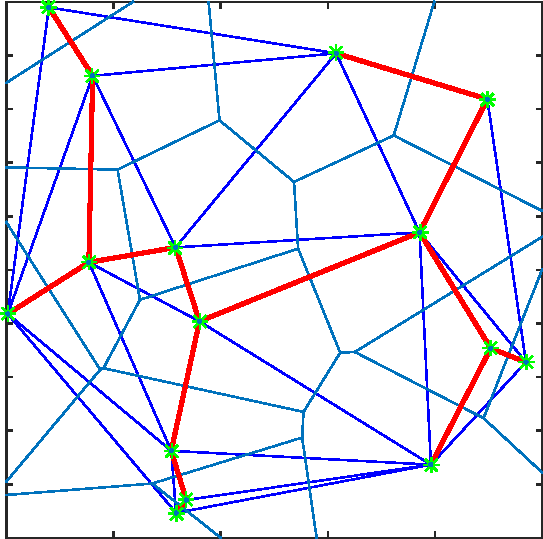
\includegraphics[width=10cm]{mst.pdf}
 \caption{Delaunay triangulation, Voronoi Diagram and Minimum spanning tree of a point process of 15 points with a uniform distribution.}
 \label{fig:point_process_voronoi:matlab:mst}
\end{figure}

Let P be a point process, generated by:
\begin{matlab}
P = rand(15,2);

% display
plot(P(:,1), P(:,2), 'g*');
axis square
\end{matlab}

\subsubsection{Delaunay Triangulation}
\begin{matlab}
DT = delaunayTriangulation(P);
triplot(DT)
\end{matlab}

\subsubsection{Voronoi Diagram}

\begin{matlab}
[V, R] = DT.voronoiDiagram();
% display
voronoi(DT);
\end{matlab}

\subsubsection{Minimum spanning tree}
\begin{matlab}
% From Delaunay Triangulation, compute edges distances
edges = DT.edges;
P1 = P(edges(:,1), :);
P2 = P(edges(:,2), :);
d = sqrt(sum((P1-P2).^2,2));

% directed graph as a sparse matrix
DG = sparse(edges(:,1), edges(:,2), d, size(P,1), size(P,1));
ST = graphminspantree(DG');
[i, j, s] = find(ST);

% display MST
for k = 1:length(i)
    plot([P(i(k),1); P(j(k),1)], [P(i(k),2); P(j(k),2)], 'r', 'linewidth', 2);
end
axis square
\end{matlab}

\subsection{Quantification}
From the previous code, the quantification is performed via the following commands:
\begin{matlab}
ad=AD(V,R);
rfh=RFH(V,R);
delaunay_parameter=[mean(d) std(d)];
mst_parameter=[mean(s) std(s)];
\end{matlab}

with
\begin{matlab}
function sol = AD(V, R )
% computes AD (Area Disorder) parameter
% V: Vertices from Voronoi
% R: Regions of Voronoi

s=[];
 for i = 1:length(R) 
    if all(R{i}~=1)   % If at least one of the indices is 1, 
                      % then it is an open region 
    s=[s;polyarea(V(R{i},1),V(R{i},2))];
    end
 end
 sol=1-(1/(1+(std(s)/mean(s))));
end
\end{matlab}
and
\begin{matlab}
function sol = RFH( V, R)
% compute RFH parameter (Round Factor Homogeneity)
% V: Vertices from Voronoi
% R: Regions of Voronoi diagram

r=[];
for i = 1:length(R)
    
    if all(R{i}~=1)   % If at least one of the indices is 1,
        % then it is an open region
        l=length(R{i});
        surface=polyarea(V(R{i},1),V(R{i},2));
        
        xv=V(R{i},1);
        yv=V(R{i},2);
        perimetre=norm([xv(1),yv(1)]-[xv(l),yv(l)]);
        for k = 1:(l-1)
            perimetre=perimetre+norm([xv(k),yv(k)]-[xv(k+1),yv(k+1)]);
        end
        r=[r;4*pi*surface/(perimetre*perimetre)];
        
    end
end

sol=1-(std(r)/mean(r));

end
\end{matlab}

The results are displayed with the next command in Fig. \ref{fig:point_process_voronoi:matlab:charac}
\begin{matlab}
figure
axis([0 1 0 1]);
axis square
hold on;
l=msigd(1);
c=msigd(2);
plot(l,c,'r*');
text(l+.02,c, '(\sigma_d,\mu_d)');

plot(ad,rfh,'g*');
text(ad+.02,rfh,'(AD,RFH)');

l=msigmst(1);
c=msigmst(2);
plot(l,c,'b*');
text(l+.02,c,'(\sigma_{MST},\mu_{MST})');

legend({'Delaunay Characterization', 'Voronoi Characterization', 'MST Characterization'})
\end{matlab}

\begin{figure}[htbp]
 \centering
 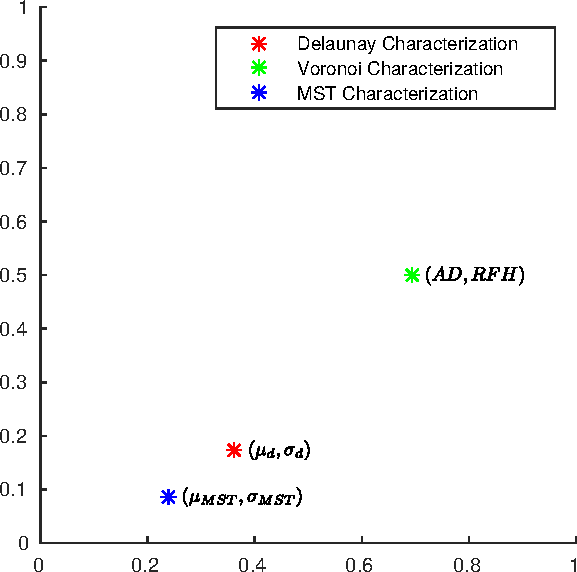
\includegraphics[width=10cm]{quantification.pdf}
 \caption{Characterization of the spatial point processes.}
 \label{fig:point_process_voronoi:matlab:charac}
\end{figure}

\subsection{Characterization of various point patterns}

\subsubsection{Regular Point Processes}
\begin{matlab}
function [x,y] = disregular(n, length)
% Regular distribution of points
% n: number of points
% length: window size
c=floor(sqrt(n));
[x2,y2]=meshgrid(0:(length/c):length,0:(length/c):length);
x=x2(:)-length/2;
y=y2(:)-length/2;
end
\end{matlab}

\subsubsection{Uniform Point Processes}
\begin{matlab}
function [x,y] = disalea( n, length )
%  uniform distribution of n points
% n: number of points
% length: window size
x1=rand(n,1);
y1=rand(n,1);
x=x1.*length-length/2;
y=y1.*length-length/2;
end
\end{matlab}

\subsubsection{Gaussian Point Processes}
\begin{matlab}
function [X,Y] = disgauss(n, length)
% generate a gaussian point process, centered in 0,0, with sigma=1;
% n: number of points
% length: window size
X=0 + randn(n,1);
Y=0 + randn(n,1);
% cut on window
X1=(-length/2<X<length/2);
X=X1.*X;
Y1=(-length/2<Y<length/2);
Y=Y1.*Y;
end
\end{matlab}

\subsubsection{Characterization}

\begin{figure}[htbp]
 \centering
 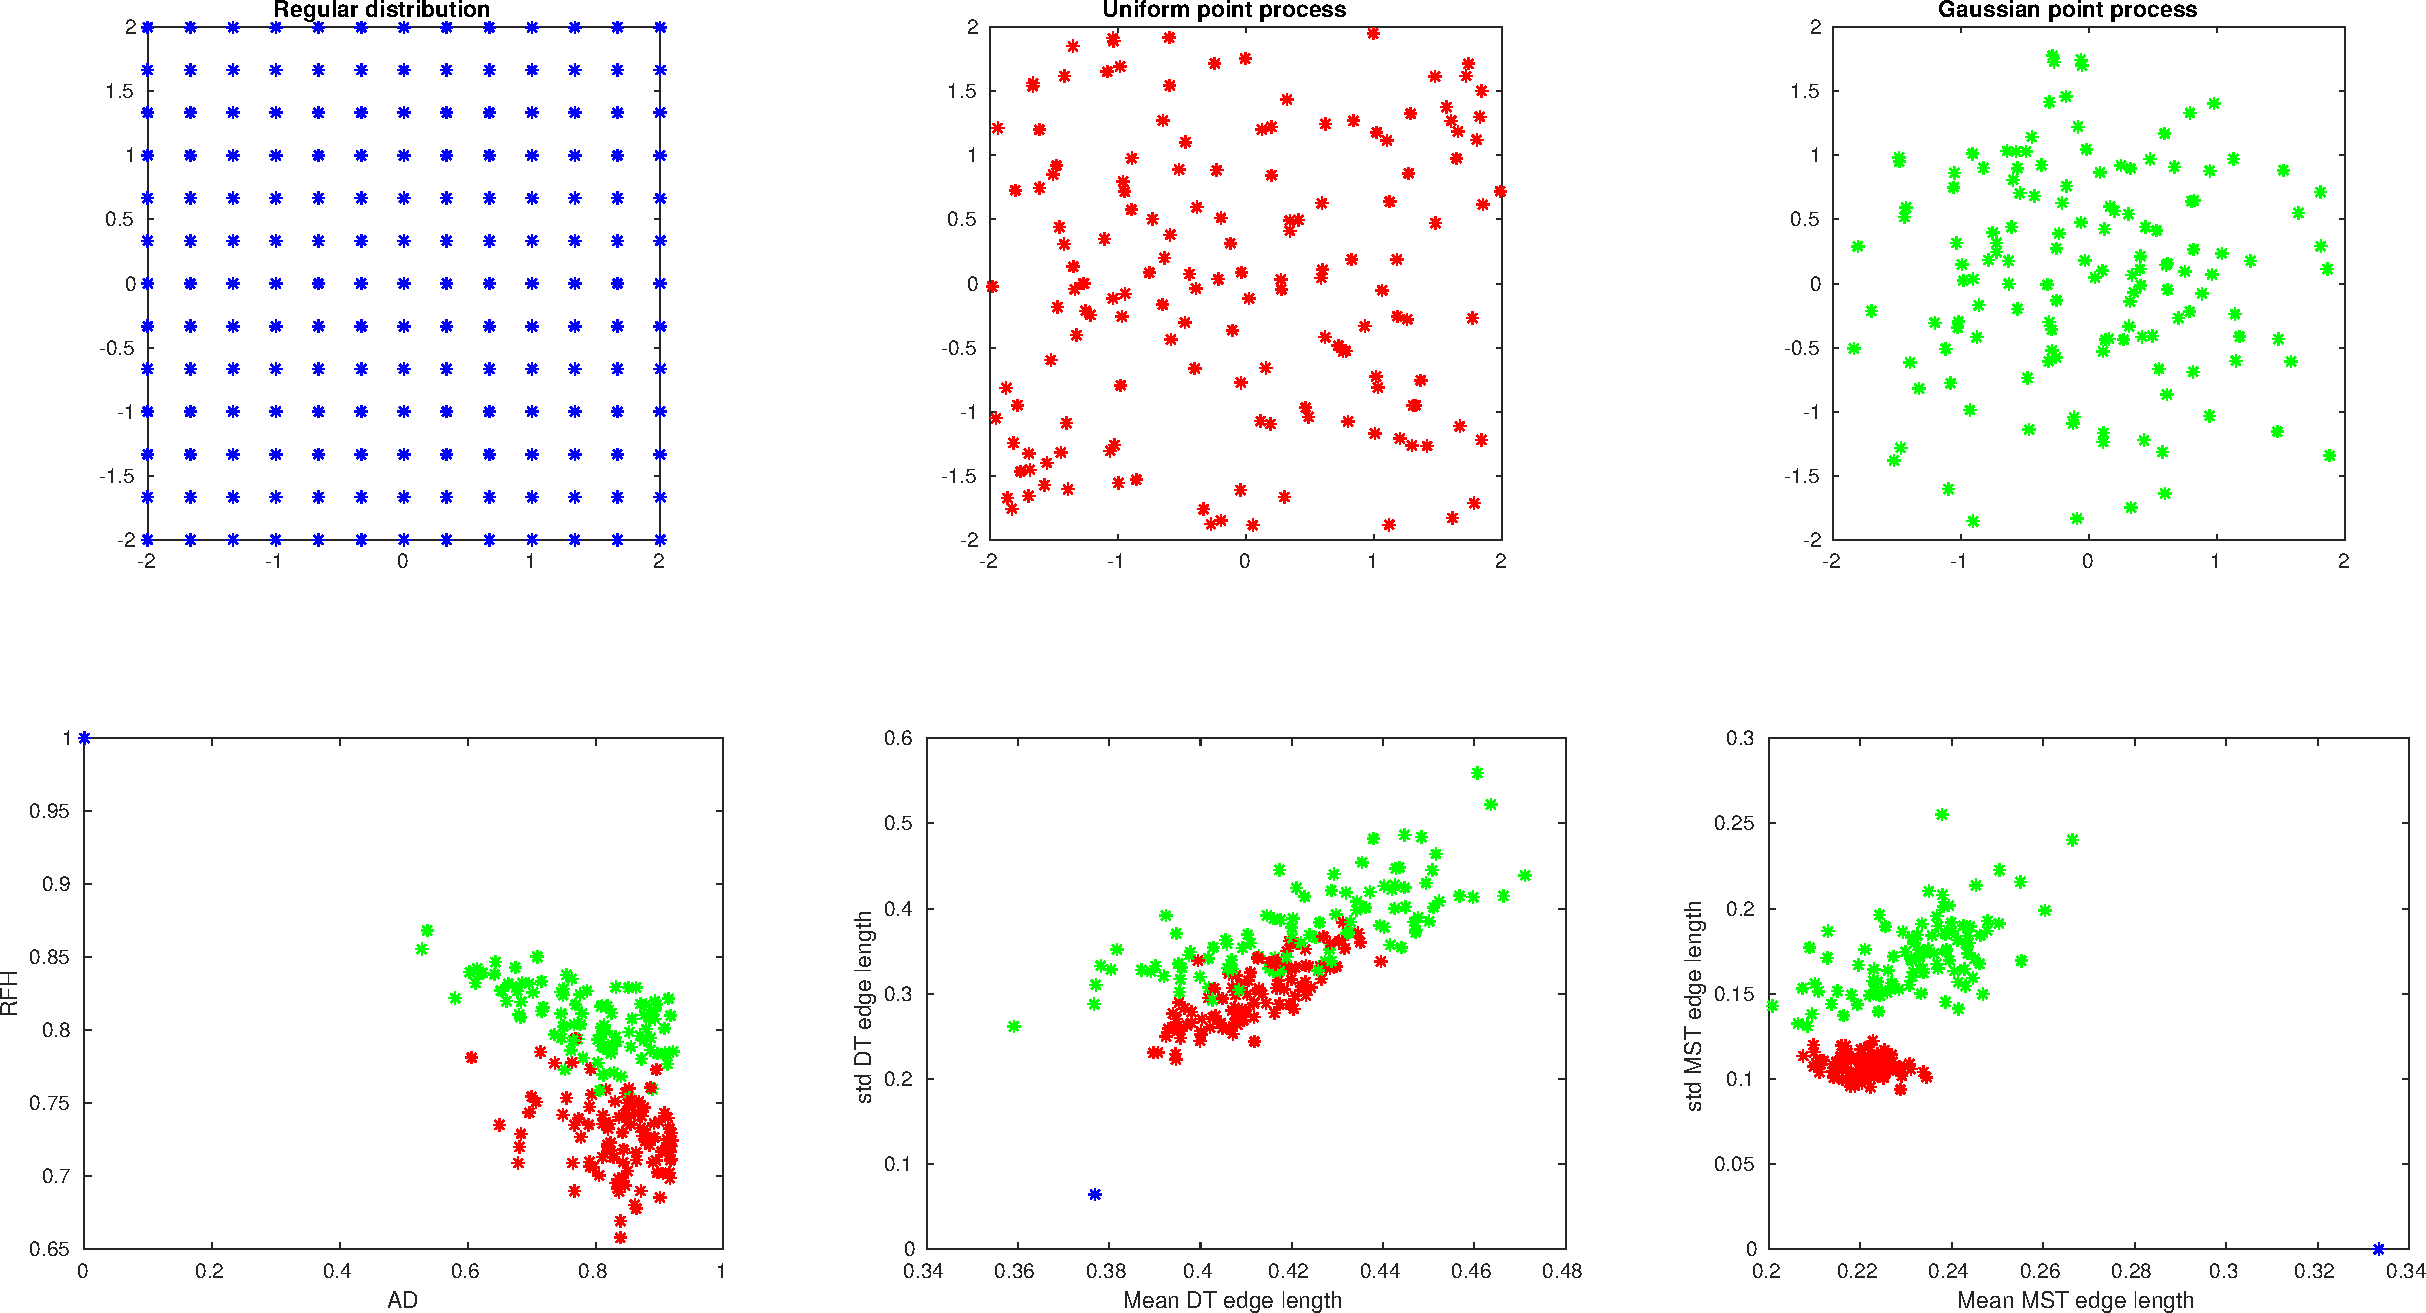
\includegraphics[width=\textwidth]{distributions.pdf}
 \caption{Characterization of different spatial point processes, with regular, uniform and gaussian distribution.}
 \label{fig:point_process_voronoi:matlab:dist}
\end{figure}

The following script generates the Fig.\ref{fig:point_process_voronoi:matlab:dist}.

\begin{matlab}
figure
[x,y]=disregular(150,4);subplot(231);plot(x,y,'b*');axis equal;title('Regular distribution');axis([-2 2 -2 2]);
 
[x,y]=disalea(150,4);subplot(232);plot(x,y,'r*');axis equal;title('Uniform point process');axis([-2 2 -2 2]);
[x,y]=disgauss(150, 4);subplot(233);plot(x,y,'g*');axis equal;title('Gaussian point process');axis([-2 2 -2 2]);
hold on

% generate 100 different processes
% display the results   
[ ad, rfh, msigd, msigmst ] = analysis( [x y], 0);
subplot(234);
axis([0 1 0 1]);
plot(ad, rfh, 'b*');  xlabel('AD'); ylabel('RFH'); hold on
subplot(235);
axis([0 1 0 1]);
plot(msigd(1), msigd(2), 'b*');  xlabel('Mean DT edge length'); ylabel('std DT edge length'); hold on
subplot(236);
axis([0 1 0 1]);
plot(msigmst(1), msigmst(2), 'b*');  xlabel('Mean DT edge length'); ylabel('std DT edge length'); hold on

for i=1:100
    [x,y]=disalea(150,4);
    [ ad, rfh, msigd, msigmst ] = analysis( [x y], 0);
    subplot(234);
    plot(ad, rfh, 'r*'); 
    subplot(235);
    plot(msigd(1), msigd(2), 'r*');
    subplot(236);
    plot(msigmst(1), msigmst(2), 'r*'); 
     
    [x,y]=disgauss(150, 8);   
    [ ad, rfh, msigd, msigmst ] = analysis( [x y], 0);
    subplot(234);
    plot(ad, rfh, 'g*');
    subplot(235);
    plot(msigd(1), msigd(2), 'g*'); 
    subplot(236);
    plot(msigmst(1), msigmst(2), 'g*'); 
    
end
\end{matlab}
